\documentclass[电力电子]{subfiles}
\begin{document}
\section{填空题}
\begin{ti}
	按内部电子和空穴两种载流子参与导电的情况,电力电子器件可分为\hua{单极型}、\hua{双极型}、\hua{复合型}三类。
\end{ti}

\begin{ti}
	电力二极管的工作特性可概括为\hua{单向导电性}。
\end{ti}

\begin{ti}
	电力二极管的主要类型有\hua{普通}、\hua{快恢复}、\hua{肖特基}。
\end{ti}

\begin{ti}
	肖特基二极管的开关损耗\hua{小于}快恢复二极管的开关损耗。
\end{ti}

\begin{ti}
	斩波电路有三种控制方式:\hua{脉宽调制}、\hua{频率调制}和\hua{混合调制}。
\end{ti}

\begin{ti}
	升压斩波电路的典型应用有\hua{直流电动机传动}和\hua{单向功率因素校正}等。
\end{ti}

\begin{ti}
	单相调压电路带电阻负载,其导通控制角 $\alpha$ 的移相范围为\hua{$0^\circ \sim 180^\circ$},随 $\alpha$ 的增大,$U_{\oo}$ \hua{逐渐减低},功率因数 $\lambda$ \hua{逐渐减低}。
\end{ti}

\begin{ti}
	单相交交变频电路带阻感负载时,哪组变流电路工作是由\hua{输出电流的方向}决定的,交流电路工作在整流还是逆变状态是根据\hua{输出电压与输出电流方向是否相同}决定的。
\end{ti}

\begin{ti}
	电流从一个支路向另一个支路转移的过程称为换流,从大的方面,换流可以分为两类,即外部换流和\hua{自换流},进一步划分,前者又包括\hua{电网换流}和\hua{负载换流}两种换流方式,后者包括\hua{器件换流}和\hua{强迫换流}两种换流方式。
\end{ti}

\begin{ti}
	PWM 控制就是对脉冲的\hua{宽度}进行调制的技术;直流斩波电路得到的 PWM 波是\hua{等效直流波形},SPWM 波得到的是\hua{等效正弦波形}。
\end{ti}

\begin{ti}
	根据载波和信号波是否同步及载波比的变化情况,PWM 调制方式可分为\hua{异步调制}和\hua{同步调制}。一般为综合两种方法的优点,在低频输出时采用\hua{异步调制}方法,在高频输出时采用\hua{同步调制}方法。
\end{ti}

\begin{ti}
	逆导晶闸管是将\hua{二极管}与晶闸管\hua{反并联}(如何连接)在同一管芯上的功率集成器件。
\end{ti}

\begin{ti}
	按照驱动电路加在电力电子器件控制端和公共端之间的性质,可将电力电子器件分为\hua{电流驱动}和\hua{电压驱动}两类。
\end{ti}

\begin{ti}
	阻感负载的特点是\hua{电流不能突变},在单相半波可控整流带阻感负载并联续流二极管的电路中,晶闸管控制角 $\alpha$ 的最大移相范围是 \hua{$180^\circ$},其承受的最大正反向电压均为 \hua{$\sqrt{2}U_{2}$},续流二极管承受的最大反向电压为\hua{$\sqrt{2}U_{2}$}(设 $U_{2}$ 为相电压有效值)。
\end{ti}

\begin{ti}
	三相半波可控整流电路中的三个晶闸管的触发脉冲相位按相序依次互差 \hua{$120^\circ$},当它带阻感负载时,$\alpha$ 的移相范围为 \hua{$90^\circ$}。
\end{ti}

\begin{ti}
	把电网频率的交流电直接变换成可调频率的交流电的变流电路称为\hua{交交变频电路}。
\end{ti}

\begin{ti}
	当采用 6 脉波三相桥式电路且电网频率为 \SI{50}{Hz} 时,单相交交变频电路的输出上限频率约为 \hua{\mbox{\SI{20}{Hz}}}。
\end{ti}

\begin{ti}
	三相交交变频电路主要有两种接线方式,即\hua{公共交流母线进线方式}和\hua{输出星形连结方式},其中主要用于中等容量的交流调速系统是\hua{公共交流母线进线方式}。
\end{ti}

\begin{ti}
	适用于全控型器件的换流方式是\hua{器件换流},由换流电路内电容直接提供换流电压的换流方式称为\hua{直接耦合式强迫换流}。
\end{ti}

\begin{ti}
	逆变电路可以根据直流侧电源性质不同分类,当直流侧是电压源时,称此电路为\hua{电压型},当直流侧为电流源时,称此电路为\hua{电流型}。
\end{ti}

\begin{ti}
	半桥逆变电路输出交流电压的幅值 $U_{\mm}$ 为 \hua{$0.5$}$U_{\dd}$,全桥逆变电路输出交流电压的幅值 $U_{\mm}$ 为 \hua{$1$}$U_{\dd}$。
\end{ti}

\begin{ti}
	三相电压型逆变电路中,每个桥臂的导电角度为 \hua{$180^\circ$},各相开始导电的角度依次相差 \hua{$120^\circ$},在任一时刻,有 \hua{3} 个桥臂导通。
\end{ti}

\begin{ti}
	PWM 波形只在单个极性范围内变化的控制方式称\hua{单极性}控制方式,三相桥式 PWM 型逆变电路采用\hua{双极性}控制方式。
\end{ti}

\begin{ti}
	根据载波和信号波是否同步及载波比的变化情况,PWM 调制方式可分为\hua{异步调制}和\hua{同步调制}。一般为综合两种方法的优点,在低频输出时采用\hua{异步调制}方法,在高频输出时采用\hua{同步调制}方法。
\end{ti}

\begin{ti}
	在如下器件:电力二极管(Power Diode)、晶闸管(SCR)、门极可关断晶闸管 GTO,属于不可控器件的是\hua{Power Diode},属于半控型器件的是\hua{SCR},属于全控型器件的是\hua{GTO}。
\end{ti}

\begin{ti}
	单相交流调压电路带阻感负载,当控制角 $\alpha < \varphi \bigl(\varphi = \arctan \frac{\omega L}{R}\bigr)$ 时,VT\textsubscript{1} 的导通时间\hua{大于\ $\uppi$},VT\textsubscript{2} 的导通时间小于 $\uppi$。
\end{ti}

\begin{ti}
	电力电子器件组成的系统,一般由控制电路、驱动电路、\hua{主电路}三部分组成。
\end{ti}

\begin{ti}
	把直流电变成交流电的电路称为\hua{逆变电路},当交流侧有电源时称为\hua{有源逆变}。
\end{ti}

\begin{ti}
	直流斩波电路完成得是直流到\hua{直流}的变换。
\end{ti}

\begin{ti}
	直流斩波电路中最基本的两种电路是降压斩波电路和\hua{升压斩波电路}。
\end{ti}

\begin{ti}
	根据载波和信号波是否同步及载波比的变化情况,PWM 调制方式可分为同步调制和异步调制。一般为综合两种方法的优点,在低频输出时采用方法是\hua{异步调制}。
\end{ti}

\begin{ti}
	电力电子器件一般工作在\hua{开关}状态。
\end{ti}

\begin{ti}
	在通常情况下,电力电子器件功率损耗主要为\hua{通态损耗},而当器件开关频率较高时,功率损耗主要为\hua{开关损耗}。
\end{ti}

\begin{ti}
	改变频率的电路称为\hua{变频电路},变频电路有交交变频电路和\hua{交直交}电路两种形式,前者又称为直接变频,后者也称为间接变频。
\end{ti}

\begin{ti}
	适用于全控型器件的换流方式是\hua{器件换流}。
\end{ti}

\begin{ti}
	对同一晶闸管,维持电流 $I_{\mathrm{H}}$ 与擎住电流 $I_{\mathrm{L}}$ 在数值大小上有 $I_{\mathrm{L}}$ \hua{大于(或 $\approx (2 \sim 4)$)}$I_{\mathrm{H}}$。
\end{ti}

\begin{ti}
	晶闸管断态不重复电压 $U_{\mathrm{DSM}}$ 与转折电压 $U_{\mathrm{BO}}$ 数值大小上应为,$U_{\mathrm{DSM}}$ \hua{小于} $U_{\mathrm{BO}}$。
\end{ti}

\begin{ti}
	电阻性负载三相半波可控整流电路中,晶闸管所承受的最大正向电压 $U_{\mathrm{Fm}}$ 等于\hua{$\sqrt{2}U_{2}$},设 $U_{2}$ 为相电压有效值。
\end{ti}

\begin{ti}
	电压型逆变器中间直流环节以\hua{电容}贮能。
\end{ti}

\begin{ti}
	三相电压型逆变电路中,每个桥臂的导电角度为\hua{$180^\circ$}。
\end{ti}

\begin{ti}
	三相半波可控整流电路中的三个晶闸管的触发脉冲相位按相序依次互差\hua{$120^\circ$}。
\end{ti}

\begin{ti}
	改变 SPWM 逆变器中的调制比,可以改变\hua{输出电压基波}的幅值。
\end{ti}

\begin{ti}
	把电网频率的交流电直接变换成可调频率的交流电的变流电路称为\hua{交交变频电路}。
\end{ti}

\begin{ti}
	$180^\circ$ 导电型电压源式三相桥式逆变电路,其换相是在\hua{同一相}的上、下二个开关元件之间进行。
\end{ti}

\begin{ti}
	晶闸管的动态参数有断态电压临界上升率 $\frac{\dd{u}}{\dd{t}}$ 和通态电流临界上升率等,若 $\frac{\dd{u}}{\dd{t}}$ 过大,就会使晶闸管出现\hua{误导通},若 $\frac{\dd{i}}{\dd{t}}$ 过大,会导致晶闸管\hua{损坏}。
\end{ti}

\begin{ti}
	三相零式可控整流电路带电阻性负载工作时,在控制角 $\alpha > 30^\circ$ 时,负载电流出现\hua{断续}。晶闸管所承受的最大反向电压为\hua{$\sqrt{6}U_{2}$}。
\end{ti}

\begin{ti}
	三相全控桥可控整流,其输出电压的脉动频率为\hua{\mbox{\SI{300}{Hz}}}。
\end{ti}

\begin{ti}
	晶闸管一旦导通,门极就失去了控制作用,故晶闸管为\hua{半控型}器件。能保持晶闸管导通的最小电流称为\hua{维持电流}。
\end{ti}

\begin{ti}
	$180^\circ$ 导电型三相桥式逆变电路,晶闸管换相是在\hua{同一桥臂}上的上、下二个元件之间进行;而 $120^\circ$ 导电型三相桥式逆变电路,晶闸管换相是在\hua{不同桥臂}上的元件之间进行的。
\end{ti}

\begin{ti}
	单相全控桥整流电路,其输出电压的脉动频率是\hua{\mbox{\SI{100}{Hz}}},三相零式可控整流电路,其输出电压的脉动频率为\hua{\mbox{\SI{150}{Hz}}}。
\end{ti}

\begin{ti}
	将直流电变为频率、电压可调的交流电称为逆变,\hua{交流测接电源}称为有源逆变。
\end{ti}

\begin{ti}
	为保证晶闸管安全可靠工作,需对它进行过电压、过电流保护及\hua{吸收电路}保护。
\end{ti}

\begin{ti}
	在 GTR 和 IGBT 两种自关断器件中,属于电压驱动的器件是\hua{IGBT},属于电流驱动的器件是\hua{GTR}。
\end{ti}

\begin{ti}
	在无源逆变器中,为使晶闸管可靠关断,常采用\hua{负载换流}和\hua{强迫换流}两种。
\end{ti}

\begin{ti}
	普通晶闸管的三个电极分别是\hua{阳极},\hua{阴极}和\hua{门极}。
\end{ti}

\begin{ti}
	$180^\circ$ 导电型三相桥式逆变电路,晶闸管换相是在\hua{同一桥臂}上的上、下二个元件之间进行;而 $120^\circ$ 导电型三相桥式逆变电路,晶闸管换相是在\hua{不同桥臂}上的元件之间进行的。
\end{ti}

\begin{ti}
	按内部电子和空穴两种载流子参与导电的情况,电力电子器件可分为\hua{单极型}、\hua{双极型}和\hua{复合型}三类。
\end{ti}

\begin{ti}
	通常变流电路实现换流的方式有\hua{器件换流}、\hua{电网换流}、\hua{负载换流}、\hua{强迫换流}四种。
\end{ti}

\begin{ti}
	晶闸管的导通条件是\hua{阳极加正向电压,门极加触发电流};关断条件是\hua{晶闸管加反向电压,使流过晶闸管的电流下降到零}。
\end{ti}

\begin{ti}
	在单相交流调压电路中,负载为电阻性时移相范围是\hua{$0^\circ \sim 180^\circ$},负载是阻感性时移相范围是\hua{$0^\circ \sim 180^\circ$}。
\end{ti}

\begin{ti}
	造成逆变失败的原因有\hua{触发电路不可靠}、\hua{晶闸管发生故障}、\hua{交流电源缺相或突然消失}、\hua{换相的裕量角不足}等几种。
\end{ti}

\begin{ti}
	逆变器按直流侧提供的电源的性质来分,可分为\hua{电压}型逆变器和\hua{电流}型逆变。
\end{ti}

\begin{ti}
	电压型三相桥式逆变电路的每只晶闸管导电的角度是\hua{$180^\circ$}度。
\end{ti}

\begin{ti}
	单相全控桥可控整流电路中功率因数 $\cos\varphi$ 比单相半波可控整流电路的功率因数提高了\hua{1}倍。各管上承受的最大反向电压为\hua{$\sqrt{2}u_{2}$}。
\end{ti}

\begin{ti}
	三相零式可控整流电路,在电阻性负载时,当控制角 $\alpha \leq 30^\circ$,每个晶闸管的导通角 $\theta = $ \hua{$120^\circ$}。此电路的移相范围为 \hua{$150^\circ$}。
\end{ti}

\begin{ti}
	把交流电能转换成直流电能称\hua{整流},把一种直流电能转换成另一种直流电能称\hua{直流斩波},而把直流电能转换成交流电能称\hua{逆变}。
\end{ti}

\begin{ti}
	IGBT 是一种新型复合器件,它的栅极具有\hua{MOSFET}器件的电压控制特性,而它的输出极 (c,e) 具有\hua{GTR}器件的导通压降低的特点。
\end{ti}

\begin{ti}
	门极可关断晶闸管(GTO),在导通后处于\hua{饱和}状态。为使它关断,所需加的反向门极电流要达到阳极电流的\huahua{$\frac{1}{5}$}。
\end{ti}

\begin{ti}
	逆变器按直流电源的性质分为电压源型及\hua{电流源}型。
\end{ti}

\begin{ti}
	目前常用的具有自关断能力的电力电子元件有\hua{电力晶体管}、\hua{可关断晶闸管}、\hua{功率场效应晶体管}、\hua{绝缘栅双极型晶体管}几种。
\end{ti}

\begin{ti}
	从晶闸管开始承受正向电压起到晶闸管导通之间的电角度称为\hua{触发}角,用\hua{$\alpha$}表示。
\end{ti}

\begin{ti}
	晶闸管在触发开通过程中,当阳极电流小于\hua{擎住}电流之前,如去掉\hua{触发}脉冲,晶闸管又会关断。
\end{ti}

\begin{ti}
	处于阻断状态的晶闸管,只有在阳极\hua{加正向电压},且在门极加正向触发电压时,才能使其开通。
\end{ti}

\begin{ti}
	造成在不加门极触发控制信号,即能使晶闸管从阻断状态转为导通状态的非正常转折有二种因素。一是阳极的电压上升率 $\frac{\dd{u}}{\dd{t}}$ 太快,二是\hua{阳极电压太高}。
\end{ti}

\begin{ti}
	单相全控桥直流电动机负载电路中,当控制角 $\alpha$ 大于不导电角 $\delta$ 时,晶闸管的导通角 $\theta = $ \hua{$\uppi$}。
\end{ti}

\begin{ti}
	将直流电能转换为交流电能又馈送回交流电网的逆变电路称为\hua{有源}逆变器。
\end{ti}

\begin{ti}
	确定最小逆变角 $\beta_{\min}$ 要考虑的三个因素是晶闸管关断时间 $t_{\mathrm{af}}$ 所对应的电角度 $\delta$,安全裕量角 $\theta_{0}$ 和\hua{换相重叠角}。
\end{ti}

\begin{ti}
	三相全控桥式有源逆变电路,每个晶闸管导通角 $120^\circ$,每隔 \hua{$120^\circ$} 产生一次换相。
\end{ti}

\begin{ti}
	电压型逆变器中间直流环节以\hua{电容}贮能。
\end{ti}

\begin{ti}
	在升压斩波电路中,已知电源电压 $U_{\dd} = \SI{16}{V}$,导通比 $\frac{t_{\mathrm{on}}}{t_{\mathrm{off}}} = 3$,则负载电压 $U_{\oo} = $ \hua{$64$} \si{V}。
\end{ti}

\begin{ti}
	三相全控桥可控整流,其输出电压的脉动频率为 \hua{\mbox{\SI{300}{Hz}}}。
\end{ti}

\begin{ti}
	三相零式可控整流电路带电阻性负载工作时,在控制角 $\alpha > 30^\circ$ 时,负载电流出现\hua{断续}。
\end{ti}

\begin{ti}
	在三相全控桥式变流电路中,控制角 $\alpha$ 与逆变角 $\beta$ 之间的关系为\hua{$\beta = 180^\circ - \alpha$}。
\end{ti}

\begin{ti}
	三相桥式不控整流电路中,整流二极管在每个输入电压基波周期内的换流次数为\hua{6}。
\end{ti}

\begin{ti}
	在三相全控桥式有源逆变电路中,直流侧输出电流电压 $U_{\dd} = $\hua{$-2.34 U_{2}$}$\cos\beta$。(电路中电感 $L$ 足够大且电流连续,设变压器二次侧相电压有效值为 $U_{2}$)
\end{ti}

\begin{ti}
	在一般的可逆直流拖动系统中,一般取最小逆变角 $\beta_{\min} = $\hua{$30^\circ \sim 35^\circ$}。
\end{ti}

\begin{ti}
	在桥式全控有源逆变电路中,理论上逆变角 $\beta$ 的范围是\hua{$0^\circ \sim 90^\circ$}。
\end{ti}

\begin{ti}
	对同一只晶闸管,维持电流 $I_{\HH}$ 与擎住电流 $I_{\LL}$ 在数值大小上有 $I_{\LL}$\hua{$<$}$I_{\HH}$。
\end{ti}

\begin{ti}
	在三相全控桥式整流电路单脉冲触发方式中,要求脉冲宽度\hua{$> 60^\circ$}。
\end{ti}

\begin{ti}
	三相全控桥式整流电路中晶闸管电流的有效值 $I_{\mathrm{V}_{1}} = $\huahua{$\frac{1}{\sqrt{3}}$}$I_{\dd}$。
\end{ti}

\begin{ti}
	单相全控桥式整流电路能否用于有源逆变电路中?\hua{能}。
\end{ti}

\begin{ti}
	电流型逆变器中间直流环节贮能元件是\hua{电感}。
\end{ti}

\begin{ti}
	三相半波可控整流电路能否用于有源逆变电路中?\hua{能}。
\end{ti}

\begin{ti}
	$180^\circ$ 导电型电压源型三相桥式逆变电路,其换相是在\hua{同一桥臂}的上、下二个开关元件之间进行。
\end{ti}

\begin{ti}
	把交流电能转换成直流电能称\hua{整流}。
\end{ti}

\begin{ti}
	从晶闸管开始承受正向电压起到晶闸管导通之间的电角度称为\hua{触发}角。
\end{ti}

\begin{ti}
	门极可关断晶闸管(GTO),为使它关断,所需加的反向门极电流要达到阳极电流的\huahua{$\frac{1}{5}$}。
\end{ti}

\begin{ti}
	正弦脉宽调制(SPWM)技术运用于电压型逆变电路中,改变\hua{载波的频率}可改变开关管的工作频率。
\end{ti}

\begin{ti}
	将直流电能转换为交流电能又馈送回交流电网的逆变电路称为\hua{有源}逆变器。
\end{ti}

\begin{ti}
	晶闸管变流器主电路要求角发电路的触发脉冲应具有一定的宽度,且前沿尽可能\hua{陡}。
\end{ti}

\begin{ti}
	电流型逆变器中间直流环节以\hua{电感}贮能。
\end{ti}

\begin{ti}
	在 PWM 斩波器中,电压比较器两个输入端信号分别是三角波信号和\hua{正弦波调制信号}。
\end{ti}

\begin{ti}
	三相半波可控整流电路中的三个晶闸管的触发脉冲相位按相序依次互差\hua{$120^\circ$}。
\end{ti}

\begin{ti}
	在电压型逆变器中,输出电压波形为\hua{方波}。
\end{ti}

\begin{ti}
	控制角 $\alpha$ 与逆变角 $\beta$ 之间的关系为\hua{$\alpha + \beta = 180^\circ$}。
\end{ti}

\begin{ti}
	单相全控桥整流电路,其输出电压的脉动频率是\hua{\mbox{\SI{100}{Hz}}}。
\end{ti}

\begin{ti}
	能保持晶闸管导通的最小电流称为\hua{维持电流}。
\end{ti}

\begin{ti}
	绝缘栅双极型晶体管的简称:\hua{IGBT},是 MOSFET 和 GTR 的复合管。
\end{ti}

\begin{ti}
	晶闸管对触发脉冲的要求是\hua{要有足够的驱动功率}、触发脉冲前沿要陡幅值要高和触发脉冲要与晶闸管阳极电压同步。
\end{ti}

\begin{ti}
	控制角 $\alpha$ 与逆变角 $\beta$ 之间的关系为\hua{$\beta = \uppi - \alpha$}。
\end{ti}

\begin{ti}
	在电流型逆变器中,输出电流波形为\hua{方波}。
\end{ti}

\begin{ti}
	型号为 KS100-8 的元件表示\hua{双向}晶闸管、它的额定电压为\hua{$800$}伏。
\end{ti}

\begin{ti}
	$180^\circ$ 导电型三相桥式逆变电路,晶闸管换相是在\hua{同一桥臂}上的上、下二个元件之间进行。
\end{ti}

\begin{ti}
	当温度降低时,晶闸管的触发电流会增加、正反向漏电流会下降;当温度升高时,正反向漏电流会\hua{增加}。
\end{ti}

\begin{ti}
	在有环流逆变系统中,环流指的是只流经逆变电源、逆变桥而不流经\hua{负载}的电流。
\end{ti}

\begin{ti}
	电力二极管的工作特性可概括为\hua{单向导电性}。
\end{ti}

\begin{ti}
	双向晶闸管的触发方式有\hua{四}种。
\end{ti}

\begin{ti}
	三相半波可控整流电路电感性负载时,电路的移相范围\hua{$0^\circ \sim 90^\circ$},三相全控桥电阻性负载时,电路的移相范围\hua{$0^\circ \sim 120^\circ$}。
\end{ti}

\begin{ti}
	直流斩波电路按照输入电压与输出电压的高低变化来分类有\hua{降压}斩波电路;\hua{升压}斩波电路;\hua{升降压}斩波电路。
\end{ti}

\begin{ti}
	晶闸管的维持电流 $I_{\HH}$ 是指在\hua{$40^\circ$}温度条件下,晶闸管从较大通态电流下降到刚好能保持导通所必须的\hua{最小}电流。
\end{ti}

\begin{ti}
	正弦脉宽调制(SPWM)技术运用于电压型逆变电路中,当改变\hua{调制波的幅值}可改变逆变器输出电压幅值;改变\hua{调制波的频率}可改变逆变器输出电压频率。
\end{ti}

\begin{ti}
	请在空格内标出下面元件的简称:电力晶体管\hua{GTR};可关断晶闸管\hua{GTO};功率场效应晶体管\hua{MOSFET};绝缘栅双极型晶体管\hua{IGBT};IGBT是\hua{MOSFET}和\hua{GTR}的复合管。
\end{ti}

\begin{ti}
	要使三相全控桥式整流电路正常工作,对晶闸管触发方法有两种,一是用\hua{宽脉冲}触发;二是用\hua{双窄脉冲}触发。
\end{ti}

\begin{ti}
	三相零式可控整流电路,在电阻性负载时,当控制角 $\alpha \leq 30^\circ$,每个晶闸管的导通角 $\theta = $\hua{$120^\circ$}。此电路的移相范围为\hua{$0^\circ \sim 150^\circ$}。
\end{ti}

\begin{ti}
	逆导晶闸管是将\hua{二极管}与晶闸管\hua{反并联}(如何连接)在同一管芯上的功率集成器件。
\end{ti}

\begin{ti}
	三相桥式全控整流电路是由一组共\hua{阳}极三只晶闸管和一组共\hua{阴}极的三只晶闸管串联后构成的,晶闸管的换相是在同一组内的元件进行的。每隔\hua{$60^\circ$}换一次相,在电流连续时每只晶闸管导通\hua{$120^\circ$}度。要使电路工作正常,必须任何时刻要有\hua{两}只晶闸管同时导通,一个是共\hua{阳}极的,另一个是共\hua{阴}极的元件,且要求不是\hua{同一桥臂}的两个元件。
\end{ti}

\begin{ti}
	电压型逆变器直流侧是电压源,通常由可控整流输出在最靠近逆变桥侧用\hua{电容}器进行滤波,而电流型逆变器直流侧是电流源,通常由可控整流输出在最靠近逆变桥侧是用\hua{电感}滤波,电压型三相桥式逆变电路换流是在\hua{同一桥臂}元件之间换流,每只晶闸管导电的角度是\hua{$180^\circ$}。
\end{ti}

\begin{ti}
	可关断晶闸管的图形符号是\hua{GTO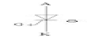
\includegraphics[width=1.5cm]{figure/fig9.png}};电力场效应晶体管的图形符号是\hua{MOSFET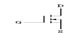
\includegraphics[width=1.5cm]{figure/fig10.png}};绝缘栅双极晶体管的图形符号是\hua{IGBT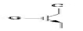
\includegraphics[width=1.5cm]{figure/fig11.png}};电力晶体管的图形符号是\hua{GTR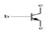
\includegraphics[width=1.5cm]{figure/fig12.png}}。
\end{ti}

\begin{ti}
	对三相桥式全控变流电路实施触发时,如采用单宽脉冲触发,单宽脉冲的宽度一般取\hua{$> 60^\circ$}度较合适;如采用双窄脉冲触发时,双窄脉冲的间隔应为\hua{$60^\circ$}度。
\end{ti}

\begin{ti}
	三相零式可控整流电路带电阻性负载工作时,在控制角 $\alpha > 30^\circ$ 时,负载电流出现\hua{断续}。晶闸管所承受的最大反向电压为\hua{$\sqrt{6}U_{2}$}。
\end{ti}

\begin{ti}
	改变 SPWM 逆变器中的调制波频率,可以改变\hua{输出波形}的频率。
\end{ti}

\begin{ti}
	在三相全控桥式变流电路中,控制角 $\alpha$ 与逆变角 $\beta$ 之间的关系为\hua{$\alpha + \beta = 180^\circ$}。
\end{ti}

\begin{ti}
	在三相全控桥式整流电路单脉冲触发方式中,要求脉冲宽度\hua{大于 $60^\circ$}。
\end{ti}

\begin{ti}
	三相桥式不控整流电路中,整流二极管在每个输入电压基波周期内的换流次数为\hua{6}。
\end{ti}

\begin{ti}
	在三相全控桥式有源逆变电路中,直流侧输出电流电压 $U_{\dd} = $\hua{$-2.34 U_{2} \cos\beta$}。(电路中电感 $L$ 足够大且电流连续,设变压器二次侧相电压有效值为 $U_{2}$)
\end{ti}

\begin{ti}
	对同一只晶闸管,维持电流 $I_{\HH}$ 与擎住电流 $I_{\LL}$ 在数值大小上有 $I_{\LL}$\hua{小于}$I_{\HH}$。
\end{ti}

\begin{ti}
	单相全控桥式整流电路能否用于有源逆变电路中?\hua{能}。
\end{ti}

\begin{ti}
	改变 SPWM 逆变器中的调制比,可以改变\hua{输出波形}的幅值。
\end{ti}

\begin{ti}
	电流型逆变器中间直流环节贮能元件是\hua{电感}。
\end{ti}

\begin{ti}
	$180^\circ$ 导电型电压源型三相桥式逆变电路,其换相是在\hua{同一桥臂}的上、下二个开关元件之间进行。
\end{ti}

\begin{ti}
	正弦脉宽调制(SPWM)技术运用于电压型逆变电路中,当改变\hua{调制比}可改变逆变器输出电压幅值。
\end{ti}

\begin{ti}
	将直流电能转换为交流电能又馈送回交流电网的逆变电路称为\hua{有源}逆变器。
\end{ti}

\begin{ti}
	三相零式可控整流电路,在电阻性负载时,当控制角 $\alpha \leq 30^\circ$,每个晶闸管的导通角 $\theta = $\hua{$120^\circ$}。
\end{ti}

\begin{ti}
	电流型逆变器中间直流环节以\hua{电感}贮能。
\end{ti}

\begin{ti}
	晶闸管的维持电流 $I_{\HH}$ 是指在 $40^\circ$ 温度条件下,晶闸管从较大通态电流下降到刚好能保持导通所必须的\hua{最小}电流。
\end{ti}

\begin{ti}
	三相半波可控整流电路中的三个晶闸管的触发脉冲相位按相序依次互差\hua{$120^\circ$}。
\end{ti}

\begin{ti}
	请在空格内标出下面元件的简称:电力晶体管\hua{GTR}。
\end{ti}

\begin{ti}
	控制角 $\alpha$ 与逆变角 $\beta$ 之间的关系为\hua{$\beta = \uppi - \alpha$}。
\end{ti}

\begin{ti}
	三相半波可控整流电路电感性负载时,电路的移相范围\hua{$0^\circ \sim 90^\circ$}。
\end{ti}

\begin{ti}
	直流斩波电路按照输入电压与输出电压的高低变化来分类有\hua{降压}斩波电路、升压斩波电路、升降压斩波电路。
\end{ti}

\begin{ti}
	三相全控桥电阻性负载时,电路的移相范围\hua{$0^\circ \sim 120^\circ$}。
\end{ti}

\begin{ti}
	请标出下面元件的简称:绝缘栅双极型晶体管\hua{IGBT}。
\end{ti}

\begin{ti}
	晶闸管变流器主电路要求角发电路的触发脉冲应具有一定的宽度,且前沿尽可能\hua{陡}。
\end{ti}

\begin{ti}
	正弦脉宽调制(SPWM)技术运用于电压型逆变电路中,改变\hua{调制波频率}可改变逆变器输出电压频率。
\end{ti}

\begin{ti}
	要使三相全控桥式整流电路正常工作,对晶闸管触发方法有两种,一是用\hua{宽脉冲}触发;二是用双窄脉冲触发。
\end{ti}

\begin{ti}
	电力二极管的工作特性可概括为\hua{单向导电性}。
\end{ti}

\begin{ti}
	控制角 $\alpha$ 与逆变角 $\beta$ 之间的关系为\hua{$\beta = \uppi - \alpha$}。
\end{ti}

\begin{ti}
	单相交交变频电路带阻感负载时,哪组变流电路工作是由\hua{输出电流的方向}决定的。
\end{ti}

\begin{ti}
	逆导晶闸管是将二极管与晶闸管\hua{反并联}(如何连接)在同一管芯上的功率集成器件。
\end{ti}

\begin{ti}
	电流从一个支路向另一个支路转移的过程称为换流,从大的方面,换流可以分为两类,即外部换流和\hua{自换流}。
\end{ti}

\begin{ti}
	按照驱动电路加在电力电子器件控制端和公共端之间的性质,可将电力电子器件分为\hua{电流驱动}和电压驱动两类。
\end{ti}

\begin{ti}
	控制角 $\alpha$ 与逆变角 $\beta$ 之间的关系为\hua{$\beta = \uppi - \alpha$}。
\end{ti}

\begin{ti}
	把电网频率的交流电直接变换成可调频率的交流电的变流电路称为\hua{交交变频电路}。
\end{ti}

\begin{ti}
	正弦脉宽调制(SPWM)技术运用于电压型逆变电路中,改变\hua{载波频率}可改变开关管的工作频率。
\end{ti}

\begin{ti}
	电压型逆变器中间直流环节以\hua{电容}贮能。
\end{ti}

\begin{ti}
	\hua{IGBT}是 MOSFET 和 GTR 的复合管。
\end{ti}

\begin{ti}
	适用于全控型器件的换流方式是\hua{器件换流}。
\end{ti}

\begin{ti}
	三相电压型逆变电路中,每个桥臂的导电角度为\hua{$180^\circ$}。
\end{ti}

\begin{ti}
	全桥逆变电路输出交流电压的幅值 $U_{\mathrm{m}}$ 为\hua{1}(填上倍数)$U_{\dd}$。
\end{ti}

\begin{ti}
	在单相半波可控整流带阻感负载并联续流二极管的电路中,其承受的最大正反向电压均为\hua{$\sqrt{2} U_{2}$}。
\end{ti}
\end{document}